\documentclass[conference]{IEEEtran}
\usepackage[ruled,vlined]{algorithm2e}
\usepackage{amsmath}
\usepackage[english]{babel} %localisation
\usepackage{caption,subcaption} %supposedly incompatible with Springer and IOP, IEEETran and ACM SIG
\usepackage{cite} %nice citations, e.g. [1--5]
\usepackage{fixltx2e} %fix latex bugs
\usepackage{graphicx}
\PassOptionsToPackage{hyphens}{url}\usepackage{hyperref} %clickable URLS
\usepackage[htt]{hyphenat} %hyphenate \texttt
\usepackage{microtype} %makes text pretty; also condenses
\usepackage{multirow} %multiple rows in tables
\usepackage{siunitx,textcomp} %\SI{value}{unit}, \si{unit}; textcomp for microtype compatibility
%\usepackage [caption=false]{subfig} %if caption/subcaption not available
% \usepackage{tikz,pgfplots} %drawings and plots
\usepackage[siunitx]{circuitikz} %circuit figures
\usepackage[T1]{fontenc} %ensure proper hyphenation and treatment of math in sentences
\usepackage{booktabs}
\bibliographystyle{IEEEtran}

\usepackage{tikz}
\usetikzlibrary{shapes}
\usepackage{verbatim}
\usepackage{listings}
\begin{document}
\lstset{defaultdialect=[x86]{Assembler}}

% paper title
% can use linebreaks \\ within to get better formatting as desired
\title{Side Channel Analysis of an Embedded/Hardware Crypto Device}

% author names and affiliations
% use a multiple column layout for up to three different
% affiliations
\author{\IEEEauthorblockN{Dallin Marshall, Sam Mitchell, and Nathanael Weidler}
\IEEEauthorblockA{Deptartment of Electrical and Computer Engineering\\
Utah Stat University\\
Logan, Utah 84322\\
e-mail: geekbott@gmail.com, samuel.alan.mitchell@gmail.com, NWeidler@gmail.com}
}

% make the title area
\maketitle


\begin{abstract}
%\boldmath
% Summarize project and results (executive summary).
%
	This paper describes the design and implementation of a physically unclonable function (PUF). One subset of PUFs is a True Random Number Generator (TRNG). We propose a compact hardware-based TRNG composed of Kumar's butterfly PUF \cite{Kumar2008}. 
 
\end{abstract}

\begin{IEEEkeywords}
Physically unclonable Function, Device Authentication.
\end{IEEEkeywords}

\section{Introduction}
	A physically unclonable function (PUF) can be used in various applications. One method is to generate testing user authentication. The server sends a challenge to a device, and the device responds using the output to the PUF; this is called a challenge response pair. If the PUF is truly unclonable, this authentication method is effectively secure. 

	The analysis of PUFs in authentication relies on 2 characteristics of the PUF: the variation between devices, $\mu_{intra}$, and the reliability of the device to reproduce the same bitstream given a challenge, $\mu_{inter}$. 

	Another type of PUF is a True Random Number Generator (TRNG). TRNGs can be used to randomly select people for jury duty, generate encryption keys, or anything else that requires randomness. 

\subsection{Related works}

	Some of the main usages of PUFs are to provide reliable device identification, device authentication, key storage, and true random number generation \cite{tehranipoor2011introduction}. 

	Not all PUFs can be implemented on every type of device (FPGA, ASIC, microcontroller). There are various types of PUFs that can be implemented on an FPGA \cite{VanHerrewege2015}, some of which are SRAM, Butterfly \cite{Kumar2008}, flip-flop \cite{Maes2008,Leest2010}, Buskeeper \cite{Simons2012}. 

	The Butterfly PUF was analyzed in \cite{morozov2010analysis} with results inconsistent with \cite{Kumar2008}. The authors determined that this was due to the difficulty to define the routing distance between gates. 


\subsection{Structure of paper}
	The organization is as follows: in Section \ref{sec::des_impl}, the development of the PUF is presented.  
	% In Section \ref{sec::expr} the experimental test setup for the capturing of the challenge response pairs is described. 
	Section \ref{sec::analysis} contains the analysis of the data. Conclusions are detailed in Section \ref{sec::conclusion}. 


\section{Design} \label{sec::des_impl}
	The butterfly PUF consists of wiring 2 NAND gates together in positive feedback mode, as shown in Figure \ref{fig:bfly}. Upon excitation, the gates are put into a race condition until the voltage level converges (less than 1 second). The butterfly should result in a consistent output for each device it's implemented on, while the output of the devices have low correlation. When implemented on a Spartan IV, the majority of the butterfly PUFs gave consistent but unique output, but the logic of 12\% never converges to one voltage. 
		\begin{figure}[tbph]
			\centering
			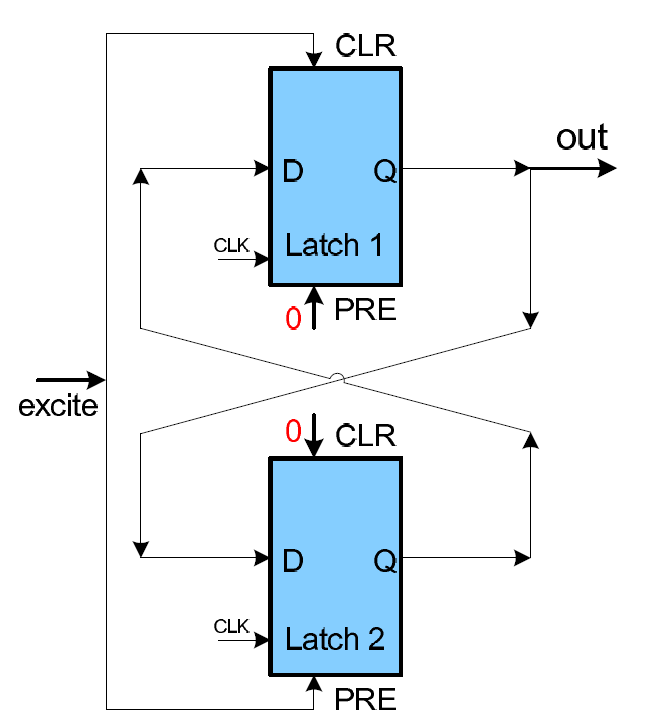
\includegraphics[width=0.3\textwidth]{bfly.png}
			\caption{Butterfly PUF: This works because of cross-coupled latches.}\label{fig:bfly}
		\end{figure}

	This paper utilizes a modified butterfly PUF that accepts an input. The excite signal is used as a switching signal through negation, as shown in Figure \ref{fig:bfly2}. This allows the PUF to accept an input, which results in 2 potential random outputs. Testing showed that some PUFs would consistently toggle, some would consistently remain 1 value, and some weren't consistent, which is consistent with the 12\% of the standard butterfly PUF that wouldn't converge. This PUF is very compact, requiring only 0.03\% of the FPGA space. 
		\begin{figure}[tbph]
			\centering
			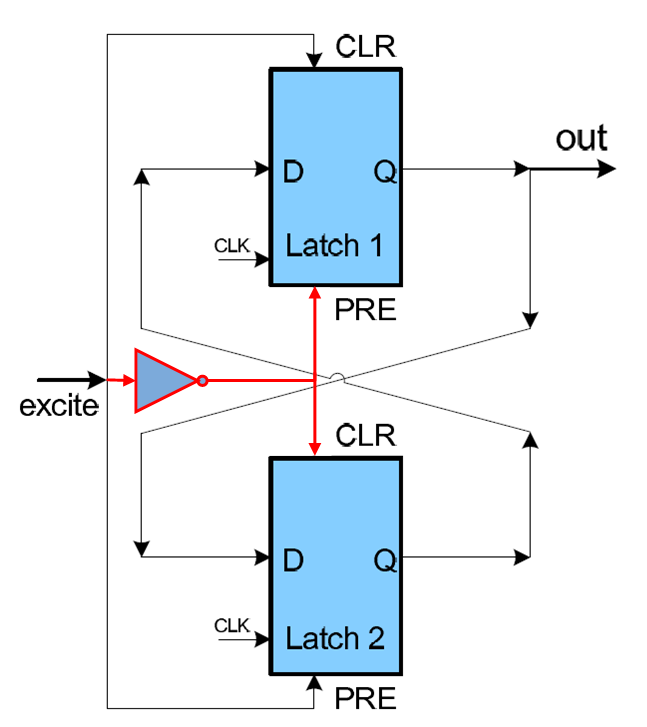
\includegraphics[width=0.3\textwidth]{bfly2.png}
			\caption{Modified-butterfly PUF: The cross-coupled latches are altered by the input.}\label{fig:bfly2}
		\end{figure}
		

	\subsection{Butterfly in authentication}
		An authentication device accepts a challenge sequence and sends back a device-specific response. We designed a modified-butterfly PUF authentication device that accepts a 64-bit key input and responds with a 64-bit key. 

		The device is a 64 by 64 grid of modified-butterfly PUFs. Each column uses an XOR gate to accept 1 bit of the 64-bit key; column 1 accepts bit 1, the output of column 1 is XORed with bit 2 and fed to column 2. The row order corresponds with the response bits; row 1 produces bit 1. 

		This design is valid because each bit of the key can alter the response up to 50\%, which means that the corresponding response bit can only be predicted with 50\% accuracy. Each row has a unique string of PUFs, so each response bit will be random to the other bits. 

		A simple verification was performed on this system by implementing 1 row of our modified-butterfly authenticator PUF. Two of the 64 stages are represented in Figure \ref{fig:bfly3}. However, unique keys did not successfully produce unique responses.  It seemed that the output was almost completely random data.  There was nothing deterministic about the result of this string of 64 butterfly PUFs.
		
		\begin{figure}[h]
			\centering
			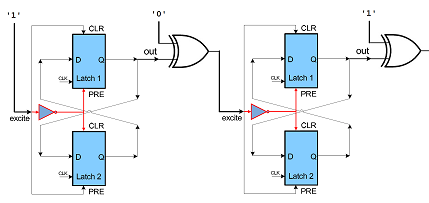
\includegraphics[width=0.5\textwidth]{bflyString.png}
			\caption{The first two stages of a 64 stage PUF.}\label{fig:bfly3}
		\end{figure}	
			
		It is believed that without manually length matching the feedback nets in FPGA editor a single indeterministic butterfly in the chain can cause the entire chain to be unstable (depending on the challenge.)  Through our testing it seems that 1 in 6 butterfly PUFs would be random.  That means in a string of 64 there are 10 or 11 that are random.  The modified-butterfly PUF was discarded for authentication applications, but a new idea emerged.

	\subsection{Butterfly in TRNG}
		TRNG requires random processes to extract numbers from. The butterfly PUF setup for this is the same as seen in Figure \ref{fig:bfly3}.  It was decided to determine if the string of 64 butterfly PUFs produced truly random data.  In order to accommodate this there were two values used to excite the 64 butterfly PUFs.  The first was the pattern "101010101010101010101010..." repeated out to 64 bits.  The second was the pattern "010101010101010101010101..." repeated out to 64 bits.  Each pattern is held for 5000 clock cycles as the butterfly is allowed to settle. The frequency of the FPGA clock is 50MHz so each value is held for 100 micro seconds.
		
		The output of the last butterfly in the string is read and if is was a '1' a 0x31 would be sent over the UART transmitter.  If it was a '0' a 0x30 would be sent over the transmitter so that the data would be simple to digest.  The transmitter was tied high so that it would always transmit.  This way the last PUF would be ringing as it settles and we would see random data.  Once the PUFs settled we would see the output settle to a value and then the PUFs would be excited again with the opposite 64 bit pattern.  This was accomplished by toggling a slide switch on the FPGA board.
		
		With a baud rate of 9600 with 8 data bits, 1 stop and 1 parity bit we get 960 bits per second output from the TRNG.  However these come in bursts of about 1000 before the butterfly settles and needs to be excited again by toggling the slide switch.  This means that the overall rate of the TRNG depends on how efficiently you can re-excite the PUFs once they settle as the constant values are discarded in between the random numbers.
		
% \section{Experimental Setup} \label{sec::expr}
	
	

\section{Data Analysis}\label{sec::analysis} 
	To verify the integrity of a TRNG we needed to verify that the steams produced by the PUF were indeed random. The two tests historically used to verify these streams were the Diehard tests and the NIST (STS) tests. Each of these test packages use multiple tests to verify the randomness of a stream. Presently, these tests are both part of the Dieharder test package, which was created to be the Swiss Army Knife of random number testing. These packages use statistical models to try and predict future numbers in the sequence.

	To test our PUF we first captured a bit stream from the PUF and saved this stream to a file. Next we ran this file through the Dieharder package. Throughout our testing phase we never had a stream that failed a single test within the the Dieharder package. There were a few false positives that the test identified with a weak correlation to a specific test. As the length of our streams increased these false positive results became much less common.This positive feedback from the Dieharder tests allowed us to feel particularly good about the viability of the modified-butterfly PUF as a TRNG.
% \section{Results}\label{res}

\section{Conclusion}\label{sec::conclusion} 
		The theory behind using a butterfly PUF for authentication is a sound theory.  However the implementation would require more time than we had for this project.  We still believe that if the lengths of the feedback nets were matched inside the FPGA for each PUF this would make a very reliable means of authentication.  This will be left to future work.
		
		The fact that butterfly PUFs are unstable for a time make them very good building blocks for TRNGs.  Our results showed that our PUF solution to the TRNG is very promising.  There could be ways to improve the design but we are pleased with the results attained above.  An improvement may be to profile the PUF and excite it again before it settles to a steady value.  This would greatly improve the rate of random number generation as you would not need to discard the steady values seen between the random values.  Also simply increasing the baud rate would increase the throughput and would be worthwhile if the other optimization was made as well.


% \nocite{*}
\bibliography{bibpuf}
% that's all folks




\end{document}






